\section{Virtualization}

This section describes some key similarities and differences between containers and
virtual machines (VMs), as well as the respective usage scenarios for VMs and containers.

\subsection{Virtual Machine (VM)}
The size of VMs is typically measured in gigabytes, e.g. the size of one
VM with a Windows 11 development environment is about 20GB.\cite{b26}
They usually contain their own operating system (OS), thus being able to perform
several resource-intensive functions at once.


\subsubsection{Structure of VM}

Unlike containers, a VM runs a full OS (including its own kernel),
as shown in the Figure 1\cite{b23}:
\begin{figure}[h!]
    \centering
    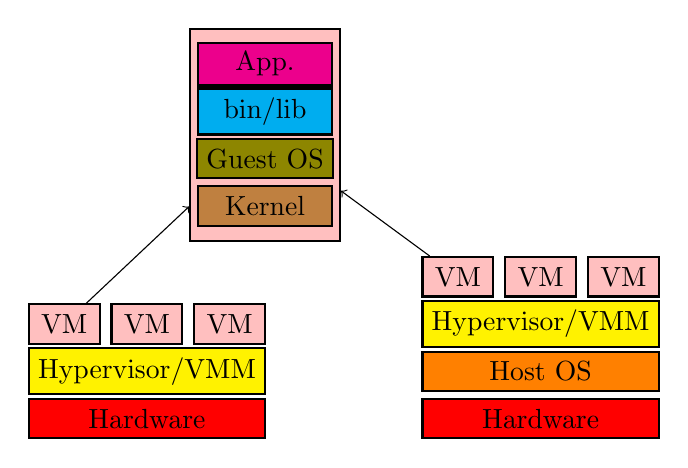
\begin{tikzpicture}
        \node [draw, thick, fill = pink, minimum width = 1.9cm, minimum height = 2.7cm]
        (vm)at(-1,3.6){};
        %App
        \node [draw, thick, fill = magenta, minimum width = 1.7cm, minimum height = 0.5cm]
        (va)at(-1,4.5){App.};
        %Bins/Lib
        \node [draw, thick, fill = cyan, minimum width = 1.7cm, minimum height = 0.5cm]
        (vb)at(-1,3.9){bin/lib};
        %Guest OS
        \node [draw, thick, fill = olive, minimum width = 1.7cm, minimum height = 0.5cm]
        (OS1)at(-1,3.3){Guest\ OS};
        %Kernel
        \node [draw, thick, fill = brown, minimum width = 1.7cm, minimum height = 0.5cm]
        (K1)at(-1,2.7){Kernel};

        %VM
        \node [draw, thick, fill = pink, minimum width = 0.9cm, minimum height = 0.5cm]
        (v1)at(-3.55,1.2){VM};
        \node [draw, thick, fill = pink, minimum width = 0.9cm, minimum height = 0.5cm]
        (v2)at(-2.5,1.2){VM};
        \node [draw, thick, fill = pink, minimum width = 0.9cm, minimum height = 0.5cm]
        (v3)at(-1.45,1.2){VM};

        \node [draw, thick, fill = pink, minimum width = 0.9cm, minimum height = 0.5cm]
        (v4)at(1.45,1.8){VM};
        \node [draw, thick, fill = pink, minimum width = 0.9cm, minimum height = 0.5cm]
        (v5)at(2.5,1.8){VM};
        \node [draw, thick, fill = pink, minimum width = 0.9cm, minimum height = 0.5cm]
        (v6)at(3.55,1.8){VM};

        %Hypervisor
        \node [draw, thick, fill = yellow, minimum width = 3cm, minimum height = 0.5cm]
        (Hyper1)at(-2.5,0.6){Hypervisor/VMM};
        \node [draw, thick, fill = yellow, minimum width = 3cm, minimum height = 0.5cm]
        (Hyper2)at(2.5,1.2){Hypervisor/VMM};

        \node [draw, thick, fill = orange, minimum width = 3cm, minimum height = 0.5cm]
        (HOS2)at(2.5,0.6){Host OS};

        \node [draw, thick, fill = red, minimum width = 3cm, minimum height = 0.5cm]
        (Infra1)at(-2.5,0){Hardware};
        \node [draw, thick, fill = red, minimum width = 3cm, minimum height = 0.5cm]
        (Infra2)at(2.5,0){Hardware};

        \draw [->](v1)--(vm);
        \draw [->](v4)--(vm);

    \end{tikzpicture}
    \caption{Structure of VM}
    \label{Structure of VM}
\end{figure}
\newline
From the bottom to the top:

1.
\textbf{Hardware}:
It is composed of CPU, Memory, Disk, NIC and other hardware.
The Hardware can be a laptop in the office, a server in a data center, or a cloud host in
an enterprise.

2.
\textbf{(Host Operating System)}:
The Host OS, which is the original OS of the device, can be installed on the
bare-metal environment (hardware).
For VM, the Host OS is not necessary, whether there is a Host OS depends on
the type of Hypervisor (Typ1 or Typ2).

3.
\textbf{Hypervisor / Virtual Machine Monitor (VMM)}:
It is an abstraction layer between the existing hardware and the other OSs that
will be installed\cite{b22}.
With a Hypervisor, it is possible to operate multiple different Guest OSs independent
of the hardware.
\newline
There are two types of hypervisors\cite{b25}.
Type 1 is based on the hardware directly and does not require prior installation
of an OS, e.g.\ HyperKit supports MacOS, and Hyper-V supports Windows.
Type 2 is based on the Host OS above the infrastructure and uses the device driver of the
OS to access the hardware, e.g.\ VirtualBox and VMWare Workstation\cite{b22}.

4.
\textbf{Kernel}
and 5.
\textbf{Guest OS}:
As shown in the figure, suppose you need to use 3 VMs.
These VMs are very large, because each of them has their own OS and kernel.
Assuming that the size of each VM is 20GB\cite{b26}, this means that they will take up 60GB
of disk space.
Even worse, at the same time they also share the host's CPU and memory.

6.
\textbf{Dependencies}:
The dependencies need to be installed to each Guest OS, i.e.\ bin and lib files
required by various Apps.

7.
\textbf{Applications}:
Apps can be operated on each Guest OS separately, i.e.\ each
App is isolated and invisible from each other.


\subsection{Container}
The size of Containers is typically measured in megabytes, e.g. the size of one
Docker Container for Windows is about 594MB.\cite{b27}
Containers do not require the separate OSs and kernels.
They are often used to encapsulate individual functions
that perform specific tasks, i.e.\ microservices\cite{b20}.

\subsubsection{Structure of Container}
According to the above mentioned, it is obvious that Containers are much simpler and smaller than VMs.
Without the Guest OS, container can save disk space and other system resources,
as shown in the Figure 2\cite{b23}:
\begin{figure}[h!]
    \centering
    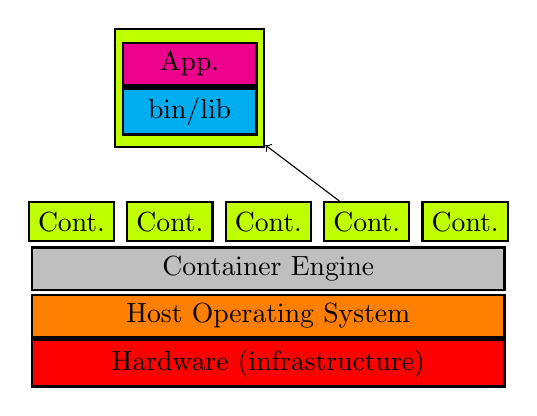
\begin{tikzpicture}
        \node [draw, thick, fill = lime, minimum width = 1.9cm, minimum height = 1.5cm]
        (cc)at(-1,3.5){};
        %App
        \node [draw, thick, fill = magenta, minimum width = 1.7cm, minimum height = 0.5cm]
        (ca)at(-1,3.8){App.};
        %Bins/Lib
        \node [draw, thick, fill = cyan, minimum width = 1.7cm, minimum height = 0.5cm]
        (cb)at(-1,3.2){bin/lib};
        %Container
        \node [draw, thick, fill = lime, minimum width = 1cm, minimum height = 0.5cm]
        (c1)at(-2.5,1.8){Cont.};
        \node [draw, thick, fill = lime, minimum width = 1cm, minimum height = 0.5cm]
        (c2)at(-1.25,1.8){Cont.};
        \node [draw, thick, fill = lime, minimum width = 1cm, minimum height = 0.5cm]
        (c3)at(0,1.8){Cont.};
        \node [draw, thick, fill = lime, minimum width = 1cm, minimum height = 0.5cm]
        (c4)at(1.25,1.8){Cont.};
        \node [draw, thick, fill = lime, minimum width = 1cm, minimum height = 0.5cm]
        (c5)at(2.5,1.8){Cont.};
        %Container Engine
        \node [draw, thick, fill = lightgray, minimum width = 6cm, minimum height = 0.5cm]
        (Hyper)at(0,1.2){Container Engine};
        \node [draw, thick, fill = orange, minimum width = 6cm, minimum height = 0.5cm]
        (HOS)at(0,0.6){Host Operating System};
        \node [draw, thick, fill = red, minimum width = 6cm, minimum height = 0.5cm]
        (Infra)at(0,0){Hardware (infrastructure)};

        \draw [->](c4)--(cc);

    \end{tikzpicture}
    \caption{Structure of Container}
    \label{Structure of Container}
\end{figure}
\newline
From the bottom to the top:

1.
\textbf{Hardware}:
Introduction as in 3.1.1

2.
\textbf{Host OS}:
All major OSs can operate containers, e.g.\ Docker.
The Host OS is necessary, which is different from the Hypervisor Type 1 of MV.

3.
\textbf{Container Engine}:
It replaces the Hypervisor to communicate directly with the Host OS and allocate
resources to respective containers.

4.
\textbf{Dependencies}:
A container encapsulates all dependencies of an App in an image, e.g.\ a Docker container
is created based on a Docker image.
When different containers share the kernel of the host OS, they cannot access it freely,
but only its virtualized view\cite{b21}.

5.
\textbf{Application}:
Different Apps are operated in different containers, they are isolated from each other.

\subsection{VM vs. Container}
For VM and container, the two most advanced virtualization methods, which is
the preferred technology?
This depends on the different application scenarios and requirements.

\subsubsection{Application Scenarios for VMs}
Because of the separate OSs, VMs occupy much more resources, the user mode of VMs is
divided into virtual user mode(User process) and the virtual kernel mode(Guest OS),
which allows VMs to run more operations.
Furthermore, due to their greater isolation, VMs can run the Apps with
business-critical data\cite{b15} and store traditional monolithic workloads\cite{b20}.

\subsubsection{Application Scenarios for Containers}
Because of the lightweight and shared OS, containers has a higher portability\cite{b20}.
They are more suitable for deploying cloud-native applications, i.e.\ a collection of
many microservices, with the aim of providing consistent development management for
Apps in a multi-cloud hybrid environment\cite{b15}.